\documentclass[10pt, conference]{FMFP2022}
% \documentclass[10pt]{article}
% \usepackage[top=1.50cm, bottom=1.50cm, left=1.884cm, right=1.884cm, includehead, includefoot, heightrounded]{geometry}
\usepackage{fancyhdr} % To use headers
\usepackage{graphicx} %To use graphics package
\usepackage[textfont=bf, font = normalsize]{caption} %To use bold and normal size font for table and figure captions
% \usepackage{floatrow} %To have table captions above the table
\usepackage{float}
\usepackage{amssymb}
\usepackage{amsfonts}
\usepackage{amsmath}
\floatstyle{plaintop} %To have table captions above the table
\restylefloat{table} %To have table captions above the table
\usepackage{subfigure} % To use subfigures
 % \floatsetup{font = normalsize} %Size of font in tables

\rhead{
    \sffamily\fontsize{9}{11}\selectfont
    \vspace{-0.5cm}
    \textbf{Proceedings of the 9th International and 49th National Conference on
      Fluid Mechanics and Fluid Power (FMFP) \\ December 14-16, 2022, IIT
      Roorkee, Roorkee-247667, Uttarakhand, India} \\ \vspace{0.15cm}
    \large{\textbf{FMFP2022-XX-YYY}}}

  % \vspace{1cm}


\usepackage{hyperref}
\usepackage{graphicx}
% \usepackage{subcaption}
\usepackage{amssymb}
\usepackage{amsmath}
\usepackage{multirow}
\usepackage{relsize}
\usepackage[utf8]{inputenc}
\usepackage{cleveref}
\usepackage{algorithm}
\usepackage[noend]{algpseudocode}
\usepackage[section]{placeins}
\usepackage{booktabs}
\usepackage{url}

% For the TODOs
\usepackage{xcolor}
\usepackage{xargs}
\usepackage[colorinlistoftodos,textsize=footnotesize]{todonotes}
\newcommand{\todoin}{\todo[inline]}
% from here: https://tex.stackexchange.com/questions/9796/how-to-add-todo-notes
% \newcommandx{\unsure}[2][1=]{\todo[linecolor=red,backgroundcolor=red!25,bordercolor=red,#1]{#2}}
% \newcommandx{\change}[2][1=]{\todo[linecolor=blue,backgroundcolor=blue!25,bordercolor=blue,#1]{#2}}
% \newcommandx{\info}[2][1=]{\todo[linecolor=OliveGreen,backgroundcolor=OliveGreen!25,bordercolor=OliveGreen,#1]{#2}}

%Boldtype for greek symbols
\newcommand{\teng}[1]{\ensuremath{\boldsymbol{#1}}}
\newcommand{\ten}[1]{\ensuremath{\mathbf{#1}}}

\usepackage{lineno}


\renewcommand{\headrulewidth}{0pt}


\begin{document}

\title{\LARGE{ \bf Fluid structure interaction with CTVF-SPH}}
\author{\textbf{Dinesh Adepu\textsuperscript{1}, Prabhu Ramachandran\textsuperscript{1}}\\\\
\textsuperscript{1}\small{Department of Aerospace Engineering, Indian Institute of
    Technology Bombay, Powai, Mumbai 400076, India}}

\maketitle
\thispagestyle{fancy}
\pagestyle{plain} % To suppress headers but still include page numbers from second page on

\noindent \textbf{ABSTRACT} In the current work we have proposed a single
unified meshless particle based numerical scheme to model fluid structure
interaction problems. A corrected transport velocity formulation is utilised to
model both fluid and solid phases. Both the phases follow the same set of
governing equations. The corrected transport velocity formulation has proved
that it has better approximation in fluids due to the corrected terms as well
the particle distribution. We also take the advantage of the ctvf scheme in
eliminating the tensile instability of the structures. The coupling is
seamlessly done as both the phases are simulated in one configuration and no
reference frame or initial frame is used to model the dynamics of any phase.
Three numerical problems are simulated to show the current scheme validation. A
clamped beam acted upon by a uniformly distributed load, hydrostatic tank on an
elastic plate, and dam breaking flow hitting a plate.
\\\\
\noindent
\textbf{Keywords:} Smoothed particle hydrodynamics; Fluid-structure interaction; Transport velocity formulation \\

\section{{\textbf{INTRODUCTION}}}

\textbf{Paragraph 1}

\begin{itemize}
\item [1] FSI is a common engineering problem, which can be seen in daily life.
  Few examples such as, the deformation of the wind turbine blade due to the
  fluid flow, and the flow traversal due to the deflected blade, blood flow in
  heart value, coastal engineering and vortex-induced vibration (Williamson and
  Govardhan, 2004; Bearman, 2011).
\item [2] Through examining the FSI, it can be utilized to optimize the systems
  and use it for better energy conservation.
\item [3] However, the coupling between the phases and the non-linearities involved
  makes it difficult to study it experimentally as well as analytically.
\item [4] This makes us to resort to numerical study, due to the flexibility of
  the study as well as it is cost efficient.
\item [5] We have meshless and mesh based schemes to model such problems. Mesh
  based schemes such as FEM, FVM are in the market for last few decades and are
  successful in modeling the FSI phenomena. But there are a few places where
  these mesh based schemes are facing difficulty, such as in free surface flow
  problems, and problems with large deformation of solids, where there is huge
  mesh distortion. Various techniques are been used to overcome such problems,
  like Immersed Boundary Method, Level set method.
\item [6] Therefore, meshless methods are used to solve problems involving free
  surface problems, and large deformation problems. As it is advantageous in
  these areas. For the past two decades several meshless methods are been
  coupled to model the fluid structure interaction. Among many meshless methods,
  we often find Smoothed particle hydrodynamics (SPH) and Material point method
  (MPM) to model the fluid phase, and the solids phase is modeled with DEM, RKPM
  or SPH itself. Few schemes with SPH and MPM are as SPH-DEM, SPH-TLSPH,
  SPH-RKPM, SPH-PD, MPM-DEM, MPM-RKPM, for more see Khayyer 2021 review paper.
  Here different phases are modeled using different numerical methods, and are
  coupled with the right boundary and interface condition. In the current work
  we use SPH alone to model fluid and solid phase.
\end{itemize}


\begin{itemize}
\item [1] SPH is particle based numerical method which was initially proposed by
  Monaghan and Lucy in 1981 to model astrophysics problems. Later it is been
  extensively applied to many other fields such as fluid flow, elastic dynamics,
  multiphase flow problems, granular flows to mention a few. For a detail review
  of SPH and its applications reader is asked to look at Monaghan 2011 paper.
\item [2] In order to model the fluid in SPH, it can be briefly classified into
  two methods. In SPH we model the fluid flow either by assuming the fluid
  as weakly compressible and incompressible.
\item [3] Though it is successful in modeling the fluid flow, SPH suffers from
  particle pairing and irregular particle distribution problem which usually
  gives rise to function approximation errors. In order to overcome such problem
  Xu et al proposed a particle shifting technique, where after each time step
  the particle positions are adjusted such that the particles are distributed
  homogeneously. And the properties are adjusted by Taylor series approximation.
  Later, Adami proposed a complete scheme where the particle transport is
  incorporated in NS equations, and a new set of equations are solved and it is
  applied to internal fluid flow problems. Zhang extended it to GTVf and solved
  free surface problems. Dinesh et al, proposed a corrected tvf scheme (CTVF)
  where the missing terms in TVF are incorporated and solved the free surface
  flow problems.
\item [4] Though it is successful in modeling the fluid flow, SPH suffers from
  particle pairing and irregular particle distribution problem which usually
  gives rise to function approximation errors. In order to overcome such problem
  Xu et al proposed a particle shifting technique, where after each time step
  the particle positions are adjusted such that the particles are distributed
  homogeneously. And the properties are adjusted by Taylor series approximation.
  Later, Adami proposed a complete scheme where the particle transport is
  incorporated in NS equations, and a new set of equations are solved and it is
  applied to internal fluid flow problems. Zhang extended it to GTVf and solved
  free surface problems. Dinesh et al, proposed a corrected tvf scheme (CTVF)
  where the missing terms in TVF are incorporated and solved the free surface
  flow problems.
\end{itemize}

\begin{itemize}
\item [1] If we consider papers, where SPH alone is used to model the fsi
  phenomena, we have WCSPH-TLSPH, WCSPH-USPH, ISPH-TLSPH. Where the coupling is
  taken care by using Adami conditions and adapted accordingly. So in all these
  schemes we have fluid being modeled in updated frame and solid being simulated
  in reference frame. No recent work has taken advantage of the transport
  velocity formulation is modeling the fsi. Where transport velocity scheme
  alone takes care of solving the tensile instability and particle distribution
  in fluids. In the current work we use CTVF to model both fluid and solid phase
  and couple them to model FSI.
\end{itemize}

\begin{itemize}
\item [1] In the current work we use CTVF to model both fluid and solid phase
  and couple them to model FSI. By using CTVF to couple both the scheme takes
  the leverage of being one consistent scheme applied for both the phases, and
  through using CTVF we were able to eliminate several numerical issues which
  arises due to the other traditional sph schemes. To test the solid solver of
  the scheme we simulate a clamped beam under a uniform loading compared against
  the analytical solution. Then for the fsi validation we simulate an aluminum
  plate under a hydrostatic tank and dam break over an elastic plate are
  simulated to validate the current solver.
\end{itemize}

\section{\textbf{METHODOLOGY}}\label{sec2}


\subsection{\textbf{Governing equations of fluid and solid media in CTVF}}\label{subsec:governing-eqtns}

The governing equations of both the fluid and the solid medium in Lagrangian form are given as,

\begin{equation}
  \label{eq:ce-tvf}
  \frac{\tilde{d} \rho}{d t} =
  - \rho \frac{\partial \tilde{u}_j}{\partial x_j} +
  \frac{\partial (\rho (\tilde{u}_j - u_j))}{\partial x_j}.
\end{equation}

\begin{equation}
  \label{eq:mom-tvf}
  \frac{\tilde{d} u_i}{d t} =
  \frac{\partial}{\partial x_j} (u_i (\tilde{u}_j - u_j))
  - u_i \frac{\partial}{\partial x_j} (\tilde{u}_j - u_j)
  + g_i
  +\frac{1}{\rho} \frac{\partial \sigma_{ij}}{\partial x_j} + \teng{f}_{fsi}.
\end{equation}
This is as per transport velocity formulation, where the particles are moved with
a transport velocity
\begin{equation}
  \label{eq:modified-material-derivative}
  \frac{\tilde{d} }{d t} = \frac{\partial }{\partial t} +
  \tilde{u}_j \frac{\partial }{\partial x_j}.
\end{equation}
with $\frac{{d} }{d t}$, $\rho$, $t$, $u_i$, $x_i$, $\sigma_{ij}$ and $g_{i}$
denoting material derivative, density, time, velocity vector, position vector,
stress tensor and gravity, respectively.


The stress tensor is split into isotropic and deviatoric parts,
\begin{equation}
  \label{eq:stress_tensor_decomposition}
  \sigma_{ij} = - p \; \delta_{ij} + \sigma'_{ij},
\end{equation}
where $p$ and $\delta_{ij}$ denote pressure and Kronecker delta function, while
$\sigma'_{ij}$ is the deviatoric stress.


For a weakly-compressible or incompressible fluid the deviatoric stress
vanishes and a viscous force is added to the stress tensor:
\begin{equation}
  \label{eq:fluid-stress-decomposition}
  \sigma_{ij} = - p \delta_{ij} + 2 \eta \frac{\partial u_i}{\partial x_j}
\end{equation}
where $\eta$ is the kinematic viscosity of the fluid.

In both fluid and solid modelling the pressure is computed using an
isothermal equation of state, given as,
\begin{equation}
  \label{eq:pressure-equation}
  p = K \bigg(\frac{\rho}{\rho_{0}} - 1 \bigg),
\end{equation}
where $K = \rho_{0} c_0^2$ is the bulk modulus. Here, the constants $c_0$ and
$\rho_0$ are the reference speed of sound and density, respectively. For solids,
$c_0$ is computed as $\sqrt{\frac{E}{3 (1 - 2 \nu)\rho_{0}}}$, $\nu$ is the
Poisson ratio.

The rate of change of deviatoric stress $\frac{d \sigma'_{ij}}{dt}$ can be
computed from the strain rate $\dot{\epsilon}_{ij}$ and rotation tensor
$\dot{\Omega}_{ij}$ according to Jaumann's formulation for Hooke's stress law
as
\begin{equation}
  \label{eq:jaumann-stress-rate}
  \frac{d \sigma'_{ij}}{dt} = 2G (\dot{\epsilon}_{ij} - \frac{1}{3}
  \dot{\epsilon}_{kk} \delta_{ij}) + \sigma^{'}_{ik}  \Omega_{jk} +
  \Omega_{ik} \sigma^{'}_{kj}.
\end{equation}
Here $G$ is the shear modulus, while $\dot{\epsilon}_{ij}$ is
\begin{equation}
  \label{eq:strain-tensor}
  \dot{\epsilon}_{ij} = \frac{1}{2} \bigg(\frac{\partial u_i}{\partial x_j} +
  \frac{\partial u_j}{\partial x_i} \bigg),
\end{equation}
and $\Omega_{ij}$ is
\begin{equation}
  \label{eq:rotational-tensor}
  \Omega_{ij} = \frac{1}{2} \bigg(\frac{\partial u_i}{\partial x_j} -
  \frac{\partial u_j}{\partial x_i} \bigg).
\end{equation}


\subsection{\textbf{Discrete equations of the fluid medium}}\label{subsec:discrete-fluid}

In the current work, both fluid and solid modelling uses the same continuity
and pressure evolution equation. The SPH discretization of the continuity
equation~\eqref{eq:ce-tvf} and the pressure evolution
equation~\eqref{eq:edac-p-evolve} respectively are,
\begin{equation}
  \label{eq:sph-discretization-continuity}
  \frac{\tilde{d}\rho_a}{dt} = \sum_{b} \; \frac{m_b}{\rho_{b}} \; (
  \rho_{a} \; \tilde{\ten{u}}_{ab} \; + \;
  (\rho \; (\tilde{\ten{u}} \; - \;
  \ten{u}))_{ab}) \; \cdot \nabla_{a} W_{ab},
\end{equation}
Here b is over both fluid solid and the structure particles (Or write b $\in$
fluid, something like that).

%
Similarly, the discretized momentum equation for fluids is written as,
\begin{multline}
  \label{eq:sph-momentum-fluid}
  \frac{\tilde{d}\ten{u}_{a}}{dt} = - \sum_{b} m_b \bigg[
  \bigg(\frac{p_a}{\rho_a^2} + \frac{p_b}{\rho_b^2}\bigg) \ten{I} -
  \bigg(\frac{\ten{A}_a}{\rho_a^2} + \frac{\ten{A}_b}{\rho_b^2} + \Pi_{ab}
  \ten{I} \bigg) \bigg]
  \cdot \nabla_{a} W_{ab} \\
  + \ten{u}_{a} \sum_{b} \frac{m_b}{\rho_{b}} \; \tilde{\ten{u}}_{ab} \cdot
  \nabla_{a} W_{ab} + \sum_{b} m_b \frac{4 \eta \nabla W_{ab}\cdot
    \ten{r}_{ab}}{(\rho_a + \rho_b) (r_{ab}^2 + 0.01 h_{ab}^2)} \ten{u}_{ab} +
  \ten{g}_{a},
\end{multline}
where $\ten{A}_a = \rho_a \ten{u}_a \otimes (\ten{\tilde{u}}_a - \ten{u}_a)$,
$\ten{I}$ is the identity matrix, $\eta$ is the kinematic viscosity of the
fluid and \cite{morris1997modeling} formulation is used to discretize the
viscosity term. $\Pi_{ab}$ is the artificial
viscosity~\cite{monaghan-review:2005} to maintain the stability of the
numerical scheme. It is given as,
\begin{align}
  \label{eq:mom-av}
  \Pi_{ab} =
  \begin{cases}
\frac{-\alpha h_{ab} \bar{c}_{ab} \phi_{ab}}{\bar{\rho}_{ab}}
  & \ten{u}_{ab}\cdot \ten{r}_{ab} < 0, \\
  0 & \ten{u}_{ab}\cdot \ten{r}_{ab} \ge 0,
\end{cases}
\end{align}
where,
%
\begin{equation}
  \label{eq:av-phiij}
  \phi_{ab} = \frac{\ten{u}_{ab} \cdot \ten{r}_{ab}}{r^2_{ab} + 0.01 h^2_{ab}},
\end{equation}
%
where $\ten{r}_{ab} = \ten{r}_a - \ten{r}_b$, $\ten{u}_{ab} = \ten{u}_a -
\ten{u}_b$, $h_{ab} = (h_a + h_b)/2$, $\bar{\rho}_{ab} = (\rho_a + \rho_b)/2$,
$\bar{c}_{ab} = (c_a + c_b) / 2$, and $\alpha$ is the artificial
viscosity parameter.



\subsection{\textbf{Solid phase modeling}}\label{subsec:solid}

\begin{equation}
  \label{eq:sph-discretization-continuity}
  \frac{\tilde{d}\rho_a}{dt} = \sum_{b} \; \frac{m_b}{\rho_{b}} \; (
  \rho_{a} \; \tilde{\ten{u}}_{ab} \; + \;
  (\rho \; (\tilde{\ten{u}} \; - \;
  \ten{u}))_{ab}) \; \cdot \nabla_{a} W_{ab},
\end{equation}


%
For solid mechanics the momentum equation is written as,
\begin{multline}
  \label{eq:sph-momentum-solid}
  \frac{\tilde{d}\ten{u}_{a}}{dt} = - \sum_{b} m_b \bigg[
  \bigg(\frac{p_a}{\rho_a^2} + \frac{p_b}{\rho_b^2}\bigg) \ten{I} -
  \bigg(\frac{\teng{\sigma}^{'}_{a}}{\rho_a^2} +
  \frac{\teng{\sigma}^{'}_{b}}{\rho_b^2} + \Pi_{ab} \ten{I} \bigg) \bigg]  \cdot \nabla_{a} W_{ab} \\
  + \ten{g}_{a},
\end{multline}
we have not considered the correction stress term $\ten{A}$ in momentum
equation of solid mechanics as it has a negligible effect.

In addition to these three equations, the Jaumann stress rate equation is also
solved. In the current work we use the momentum velocity $\ten{u}$ rather than
$\tilde{\ten{u}}$ as in the GTVF~\cite{zhang_hu_adams17} in the computation of
gradient of velocity. The SPH discretization of the gradient of velocity is
given as,
\begin{equation}
  \label{eq:sph-vel-grad}
  \nabla \ten{u}_a =
  - \sum_{b} \frac{m_b}{\rho_{b}} (\ten{u}_{a} - \ten{u}_{b}) \otimes (\nabla_{a} W_{ab}),
\end{equation}
where $\otimes$ is the outer product.

The SPH discretization of the modified Jaumann stress rate
\cref{eq:modified-jaumann-stress-rate} is given as,
\begin{multline}
  \label{eq:sph-modified-jaumann-stress}
  \frac{\tilde{d}\teng{\sigma}^{'}_{a}}{dt} = 2G (\dot{\teng{\epsilon}}_{a} -
  \frac{1}{3} \dot{\teng{\epsilon}}_{a} \ten{I}) + \teng{\sigma}^{'}_{a}
  \teng{\Omega}_{a}^{T} +
  \teng{\Omega}_{a} \teng{\sigma}^{'}_{a}
\end{multline}



\subsection{\textbf{Transport velocity computation}}\label{subsec:transport-velocity}


The particles in the current scheme are moved with the transport velocity,
\begin{equation}
  \label{eq:transport_velocity_position_derivative}
  \frac{d\ten{r}_a}{dt} = \ten{\tilde{u}}_a.
\end{equation}
%
The transport velocity is updated using,
\begin{equation}
  \label{eq:transport_velocity}
  \ten{\tilde{u}}_a(t + \Delta t) =\ten{u}_a(t) + \Delta t \; \frac{\tilde{d} \ten{u}_a}{dt} +
  \bigg(\frac{d \ten{u}_{a}}{dt}\bigg)_{\text{c}} \Delta t
\end{equation}

Where $\big(\frac{d \ten{u}_a}{dt}\big)_{\text{c}}$ is the homogenization
acceleration which ensures that the particle positions are homogeneous. In the
current work we have explored two kinds of homogenization accelerations, one
is a displacement based technique due to \cite{sun2017deltaplus}, and the
other is the iterative particle shifting technique due to
\cite{huang_kernel_2019}. These are discussed in the following.



In \cite{sun2017deltaplus}, the particle shifting technique was implemented as
a particle displacement ($\delta \ten{r}$). This was modified in
\cite{sun_consistent_2019} to be computed as a change to the velocity. In the
present work we modify this to be treated as an acceleration to the particle
in order to unify the treatment of different PST methods.

Firstly, the velocity deviation based equation is given as,
\begin{equation}
  \label{eq:sun2019_pst}
  \delta \ten{u}_a = - \text{Ma} \; (2h) c_0 \sum_b \bigg[
  1 + R \bigg( \frac{W_{ab}}{W(\Delta x)} \bigg)^n  \bigg] \nabla_a W_{ab} V_b,
\end{equation}
%
it is modified to force based as,
\begin{equation}
  \label{eq:sun2019_pst}
  \bigg(\frac{d \ten{u}_a}{dt}\bigg)_{\text{c}} = - \frac{\text{Ma} \;
    (2h) c_0}{\Delta t} \sum_b \bigg[1 + R \bigg( \frac{W_{ab}}{W(\Delta x)} \bigg)^n
  \bigg] \nabla_a W_{ab} V_b,
\end{equation}
where $R$ is an adjustment factor to handle the tensile instability, and
$\text{Ma}$ is the mach number of the flow. $V_b$ is the volume of the
$b$\textsuperscript{th} particle. The acceleration is changed to account for
particles that are on the free surface. We use $R = 0.2$ and $n = 4$ as
suggested by \cite{sun_consistent_2019}.



In \cite{sun2017deltaplus}, the particle shifting technique was implemented as
a particle displacement ($\delta \ten{r}$). This was modified in
\cite{sun_consistent_2019} to be computed as a change to the velocity. In the
present work we modify this to be treated as an acceleration to the particle
in order to unify the treatment of different PST methods.

Firstly, the velocity deviation based equation is given as,
\begin{equation}
  \label{eq:sun2019_pst}
  \delta \ten{u}_a = - \text{Ma} \; (2h) c_0 \sum_b \bigg[
  1 + R \bigg( \frac{W_{ab}}{W(\Delta x)} \bigg)^n  \bigg] \nabla_a W_{ab} V_b,
\end{equation}
%
it is modified to force based as,
\begin{equation}
  \label{eq:sun2019_pst}
  \bigg(\frac{d \ten{u}_a}{dt}\bigg)_{\text{c}} = - \frac{\text{Ma} \;
    (2h) c_0}{\Delta t} \sum_b \bigg[1 + R \bigg( \frac{W_{ab}}{W(\Delta x)} \bigg)^n
  \bigg] \nabla_a W_{ab} V_b,
\end{equation}
where $R$ is an adjustment factor to handle the tensile instability, and
$\text{Ma}$ is the mach number of the flow. $V_b$ is the volume of the
$b$\textsuperscript{th} particle. The acceleration is changed to account for
particles that are on the free surface. We use $R = 0.2$ and $n = 4$ as
suggested by \cite{sun_consistent_2019}.


\subsection{\textbf{Coupling between fluid and solid phase}}\label{subsec:fsi}
Coupling is handled straight forwardly in SPH. While modelling the fluid phase
and treating the fluid-structure interactions, the structure particles are
assumed to be boundary particles. And from the boundary handling given in
Adami [14], we compute the pressure of the boundary particles from the
extrapolated equation (12) and correspondingly set its density using equation
(13). Please note that the pressure we set here are only pertaining to the fsi
force and does not correspond to the real pressure or density of the structure
particles.

The force acting on the fluid particles is now computed from the pressure set
using the adami boundary conditions and density set consequently. We mark
particles comprising the solid as $a$ and fluid as $i$, and the force acting
on the fluid particle $i$ is given as

\begin{equation}
  f_i^s = -m_i \sum_{a} m_a \bigg(\frac{p_i}{\rho_{i}^2} +
  \frac{p_a}{\rho_{a}^2} + \Pi_{ia} \bigg) \nabla_{i} W(x_{ia})
\end{equation}

Force on the structure particle due to the fluid particle computed using
Newton's third law. Since each structure particle experiences equal and
opposite force as experienced by the fluid particle, the expression for the
force on structure due to a fluid particle is

\begin{equation}
  f_a^F = -m_i \sum_{a} m_a \bigg(\frac{p_a}{\rho_{a}^2} +
  \frac{p_i}{\rho_{i}^2} + \Pi_{ai} \bigg) \nabla_{a} W(x_{ai})
\end{equation}


One more way of coupling is by using \cite{khayyer2018enhanced} formulation.


\subsection{\textbf{Integrator}}\label{subsec:integrator}


\section{\textbf{RESULTS AND DISCUSSION}}\label{sec3}

% =========================================
% =========================================
% start
% =========================================
% =========================================
\subsection{Uniformly distributed loading on a clamped beam}
\label{sec:udl}

\begin{itemize}
\item [1] In the current section we validate the structural part of the current solver.
\item [2] We chose a homogeneous elastic plate clamped on both ends which is
  acted upon by a uniformly distributed load (q Nm$\textsuperscript{-1}$).
\item [3] The numerical solution of the y-displacement at the center of the beam
  is compared against the analytical counterpart. Where the analytical solution
  is given by.
\item [4] The schematic of the beam with a udl including the dimensions is
given in figure xx.
\item [5] The schematic of the beam with a udl including the dimensions is
shown in figure \Cref{fig:udl-schematic}.
\item [6] The material properties of the beam are, a density of 1230 kgm3, with
  an Young's modulus of 20 Pa, and a Poisson ratio of 0.
\item [7] We consider three particle resolutions such that we get 10, 15 and 20
  particles along the width directing of the beam.
\item [8] We run a total physical time of 2 sec.
\end{itemize}

% The mechanical properties of the material under consideration are as follows: an
% Young's modulus of $2.4 \times 10^{7}$ Pa with a Poisson ratio of $0$. The
% density of the material is taken as $1100$ kgm$\textsuperscript{-3}$. A total of
% three particle spacing are considered: $0.0012$ m, $0.0008$ m, $0.0006$ m which
% corresponds to $10, 15, 20$ particle layers in width direction of the beam. An
% artificial viscosity of $2$ is used in the current problem in order to stabilize
% the scheme. A total time of $2$ sec physical time is run.
\begin{figure}[!htpb]
  \centering
  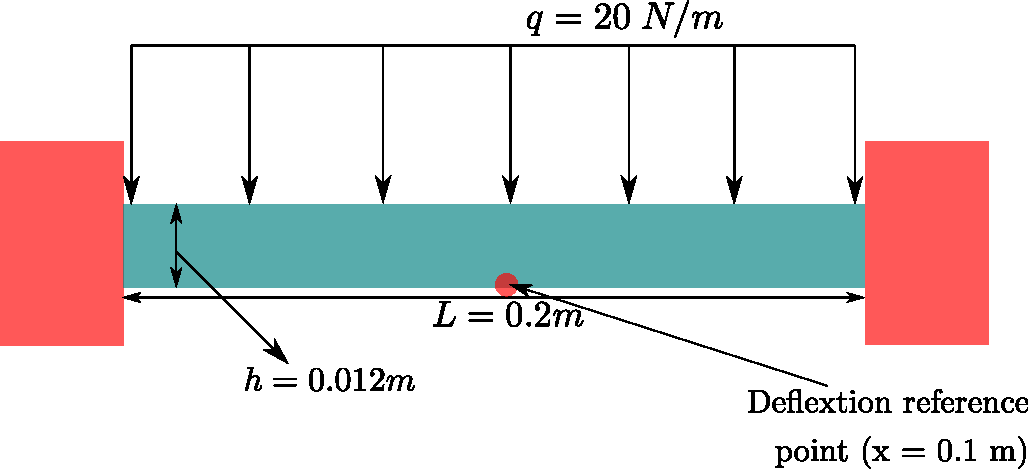
\includegraphics[scale=0.5]{images/khayyer_2021_udl/schematic}
  \caption{Schematic}
\label{fig:udl-schematic}
\end{figure}


\begin{figure}[H]
  \centering
  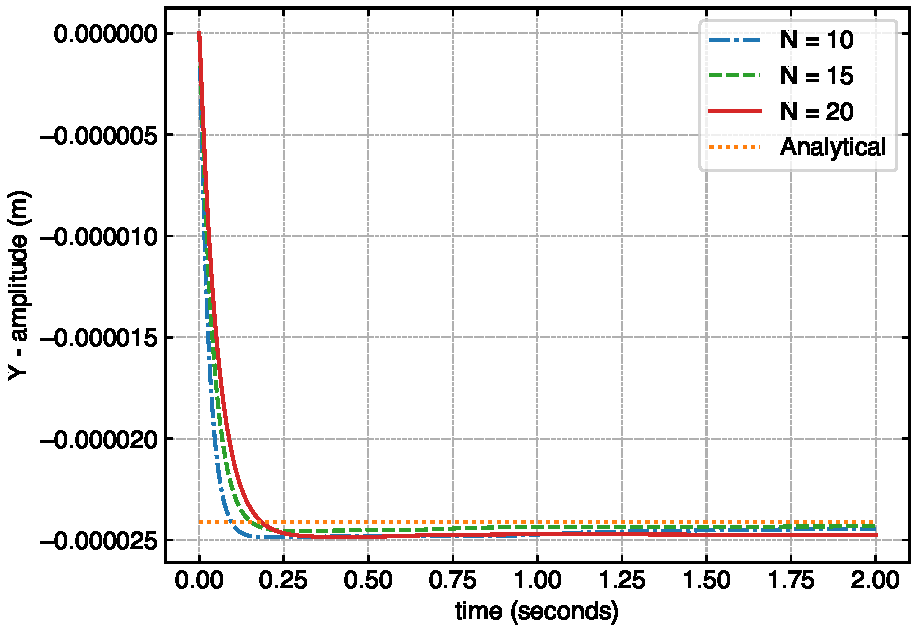
\includegraphics[scale=0.5]{figures/khayyer_2021_udl/homogenous}
  \caption{Schematic}
\label{fig:udl-disp-plot}
\end{figure}
\begin{itemize}
\item [1] \Cref{fig:udl-disp-plot} depicts the time history of y-displacement of
  the beam center for different particle resolutions computed using the current
  solver compared against the analytical solution.
\item [2] From \cref{fig:udl-disp-plot} we can see that the current solver is
  able to predict the displacement of the clamped beam accurately.
\item [3] Also as the particle spacing is reduced, the beam displacement
  is converging as well.
\end{itemize}



\subsection{Ng 2020 Hydrostatic water column on an elastic plate}
\label{sec:hydrostatic-water-column-on-an-composite-elastic-plate}

\begin{itemize}
\item [1] In this example we study the elastic deformation an elastic plate
  due to the hydrostatic tank.
\item [2] We utilise the current example to validate the current solvers ability
  in solving the fluid structure interaction problems.
\item [3] This is a famous example and is used by many solvers in the SPH
  community to validate their solvers, such as xx, xx, xx.
\item [4] The numerical solution of the y-displacement at the center of the beam
  is compared against the analytical counterpart. Where the analytical solution
  is given by.
\item [5] The schematic of fluid with the elastic beam is shown in figure xxxx.
  Along with the initial pressure distribution in the fluid.
  The figure includes the dimensions as well.
\item [7] The material properties of the beam are, a density of 1230 kgm3, with
  an Young's modulus of 20 Pa, and a Poisson ratio of 0.
\item [8] The material properties of the fluid are, a density of 1000 kgm3, with
  a dynamic viscosity of 0.
\item [9] We consider two particle resolutions such that we get 10, 15 and 20
  particles along the width directing of the beam.
\item [10] We run a total physical time of 2 sec.
\end{itemize}
% In the first example, a hydrostatic water column on an elastic plate is
% considered. The initial setup of the system with water pressure is shown in
% figure, where an initial column of fluid under hydrostatic state is rested on an
% elastic plate under gravity. The water column is $2$ m in height and $0.5$ m in
% width, while the elastic plate is of $0.05$ m in thickness and $0.5$ m in
% length, respectively. The elastic plate considered here is made of Aluminium,
% whose material properties are: Young's modulus $E = 67.5$ GPa, Poisson's ratio
% $\nu = 0.4$. According to the analytical solution \cite{sfsfd}, the deflection
% magnitude at mid-span after the system's equilibrium state is
% $d = -6.85 \times 10^{-5}$ m.
\begin{figure}[H]
  \centering
  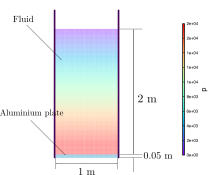
\includegraphics[scale=0.4]{images/ng_2020_hydrostatic_water_column_on_elastic_plate/schematic}
  \caption{Hydrostatic water column on an elastic plate}
\label{fig:hs-water-on-plate}
\end{figure}

%

% The simulation is ran for a total time of $0.4$ seconds. For convergence study,
% a two particle resolutions are studied, $0.35 \times 10^{-2}$ m, and
% $0.25 \times 10^{-2}$ m. These particle spacing generates $15$ and $20$
% particles along the width on the structure respectively. The test case is ran
% for a period of 0.3 seconds with 1232233 particles for the highest resolution.
% The time step of the fluid and solid phase are computed separately as per
% equation \eqref{eq:time_step}, but we use substepping to update the fluid and
% solid phases as per section \ref{section:substepping}.

\begin{itemize}
\item [1] Figure shows the snapshot of the fluid with the elastic solid, along
  with particles of the fluid having contour of the pressure. This snapshot
  corresponds to the spacing of 100.
\item [2] From the figure we can see that the current solver is able to produce
  smooth pressure distribution in the fluid.
\end{itemize}

\begin{itemize}
\item [1] \Cref{fig:udl-disp-plot} depicts the time history of y-displacement of
  the beam center for different particle resolutions computed using the current
  solver compared against the analytical solution.
\item [2] From \cref{fig:udl-disp-plot} we can see that the current solver is
  able to predict the displacement of the clamped beam accurately.
\item [3] Also as the particle spacing is reduced, the beam displacement
  is converging as well.
\end{itemize}
\begin{figure}[H]
    \centering
    \subfigure[H]
    {
      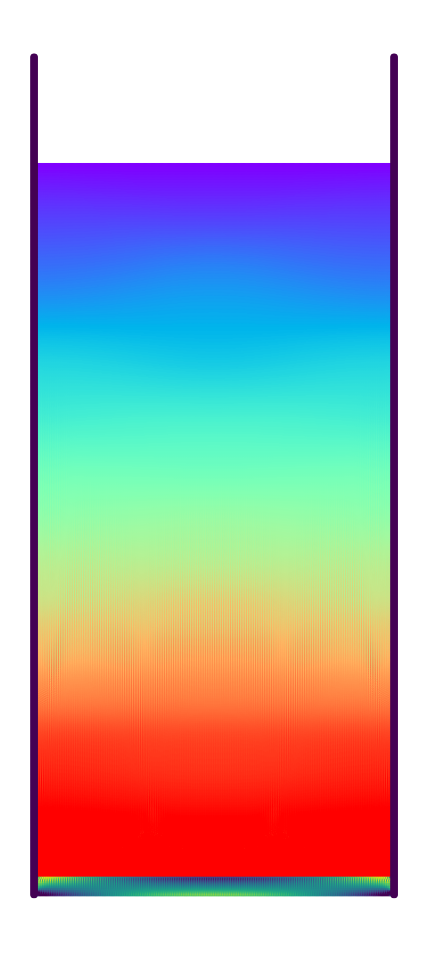
\includegraphics[scale=1.0]{figures/ng_2020_hydrostatic_water_column_on_elastic_plate/snap_t_0}
    }
    \qquad
    \subfigure[H]
    {
      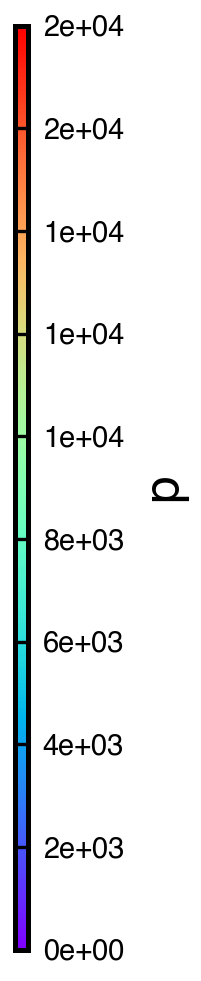
\includegraphics[scale=1.0]{figures/ng_2020_hydrostatic_water_column_on_elastic_plate/colorbar_t_0}
    }
    \caption
    {
        (a) blah
        (b) blah
    }
    \label{fig:foobar}
\end{figure}

%
\begin{figure}[H]
  \centering
  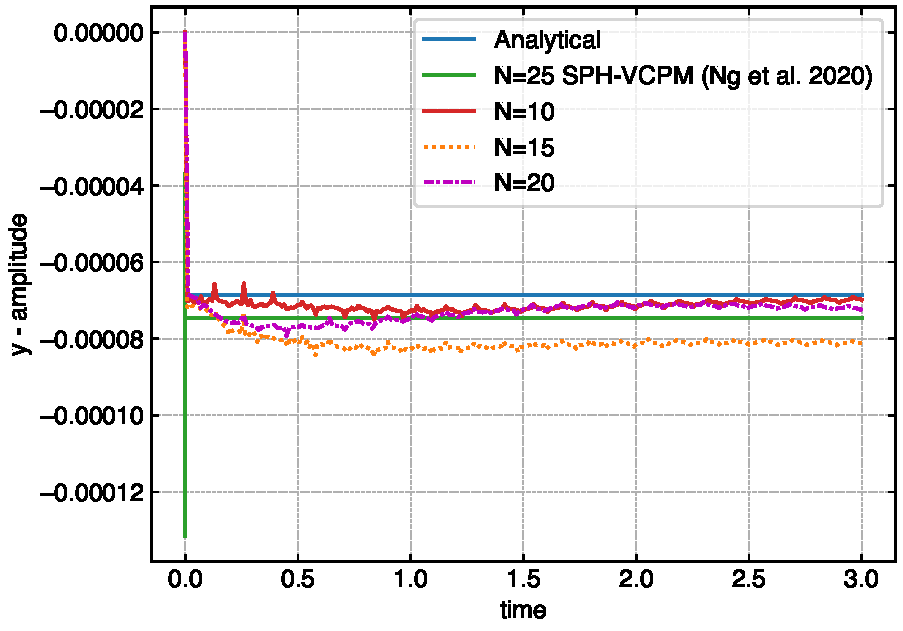
\includegraphics[scale=0.5]{{{figures/ng_2020_hydrostatic_water_column_on_elastic_plate/y_amplitude}}}
  \caption{The mid-span deflection of the structure with time}
\label{fig:ng2020hsplate:deflection}
\end{figure}
%


\subsection{Water impact onto a forefront elastic plate}
\label{sec:water-impact-forefront}
\begin{itemize}
\item [1] In the current case we study the deformation of the elastic plate due
  to the water impact of the dam breaking flow.
\item [2] This example has a experimental result to compare with.
\item [2] Here the fluid is initially released which attains a certain velocity
  by the time it impacts the structure. The structure will obstruct the fluid
  making it rise similarly the fluid will deform the elastic plate. The fluid
  will rise and hit the other end of the dam, following it comes back and hits
  the structure from back.
\item [3] We compare the current solver results to the other numerical techniques
  like qs, sph, dem, pfem.
\item [4] The initial positions of the fluid as well as the structure inside the
  dam are shown in figure figure xxxx.
\item [5] The material properties of the beam are, a density of 1230 kgm3, with
  an Young's modulus of 20 Pa, and a Poisson ratio of 0.
\item [6] The material properties of the fluid are, a density of 1000 kgm3, with
  a dynamic viscosity of 0.
\item [7] A particle spacing of xx is taken, resulting in a total of 1234
  particles, which includes fluid, structure and solid wall.
\item [8] We run a total physical time of 2 sec.
\end{itemize}
% this example the elastic plate is placed at the end. Which gets impacted due
% to the moving fluid. Further information can be found at section 3.2 of
% \cite{liu2013numerical}, \cite{sun2019fully}, {A $\delta$ SPH-SPIM coupled
%   method for fluid-structure interaction problems}.

% This case deals wit the dam-break water
% flow impact an elastic plate placed at a certain distance. \todo{Describe more
%   about how the flow evolves with time}. The initial configuration is depicted
% in \cref{fig:dam-break-flow-impact-plate-initial-setup}. The density and dynamic
% viscosity of the water are taken as $1000$ kgm$\textsuperscript{-3}$ and $0.001$
% kgm$\textsuperscript{-3}$ (These values should be changed). The particle spacing
% is set to $5 \times 10^{-4}$ m. The material properties of the elastic plate
% are: Young's modulus $E=12 MPa$ and Poisson ratio $\nu = 0.0$, with density set
% to $2000$ kgm$\textsuperscript{-3}$. The x-displacement of the plate's free end
% is recorded as time progresses. The simulation is executed for a total time of
% $t = 0.7$ s.
\begin{figure}[H]
  \centering
  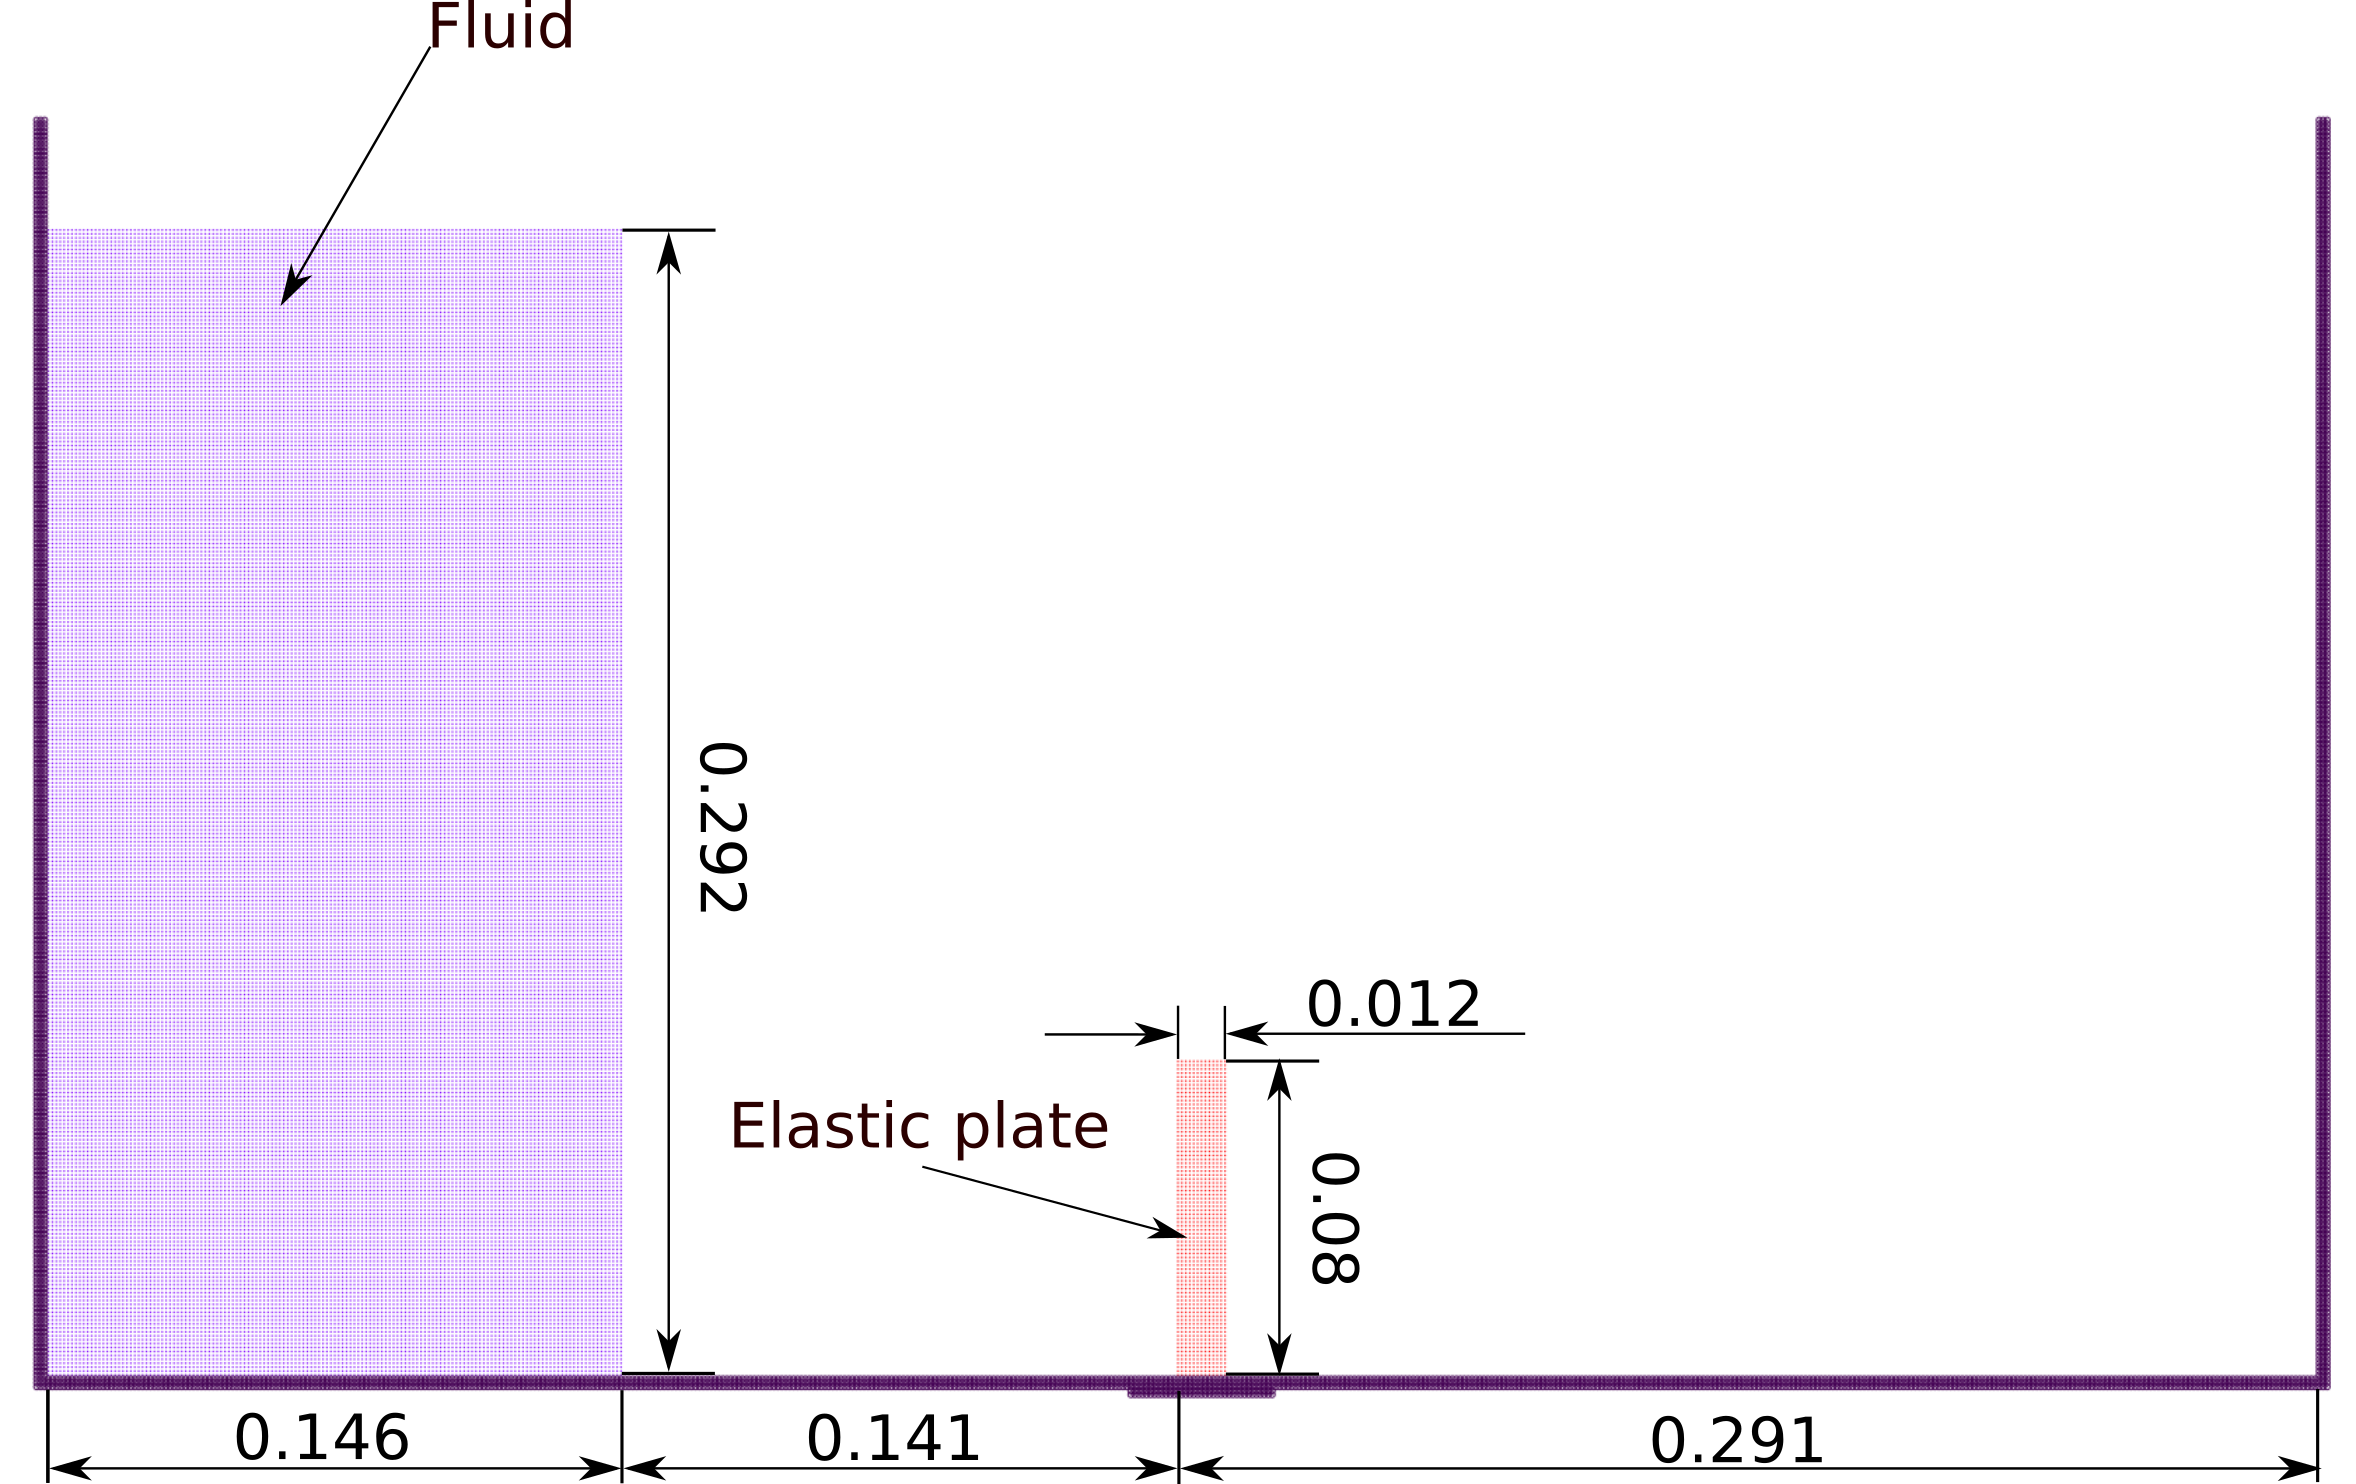
\includegraphics[scale=0.4]{images/sun_2019_dam_breaking_flow_impacting_an_elastic_plate/schematic}
  \caption{Dam-break flow impacting an elastic plate.}
\label{fig:dam-break-flow-impact-plate-initial-setup}
\end{figure}

\begin{itemize}
\item [1] Figure xx shows the snapshots of the fluid and the elastic structure
  at five time instances.
\item [2] From the snapshots we can see that the fluid after hitting the
  structure rises and hits the other end of the tank and travels back and hits
  the structure again.
\item [3] For quantitative validation we plot the x-displacement of the free end
  of the elastic structure. Figure xx, depicts the x-displacement vs time of the
  elastic structure using the current solver, against experimental result, as
  well as with other numerical results such as qs, sph, PFEM.
\item [3] From the figure xx, we can see that the displacement computed by the
  current solver is closer to the experimental as well as other numerical results.
\end{itemize}
\begin{figure}[H]
    \centering
    \subfigure[]
    {
        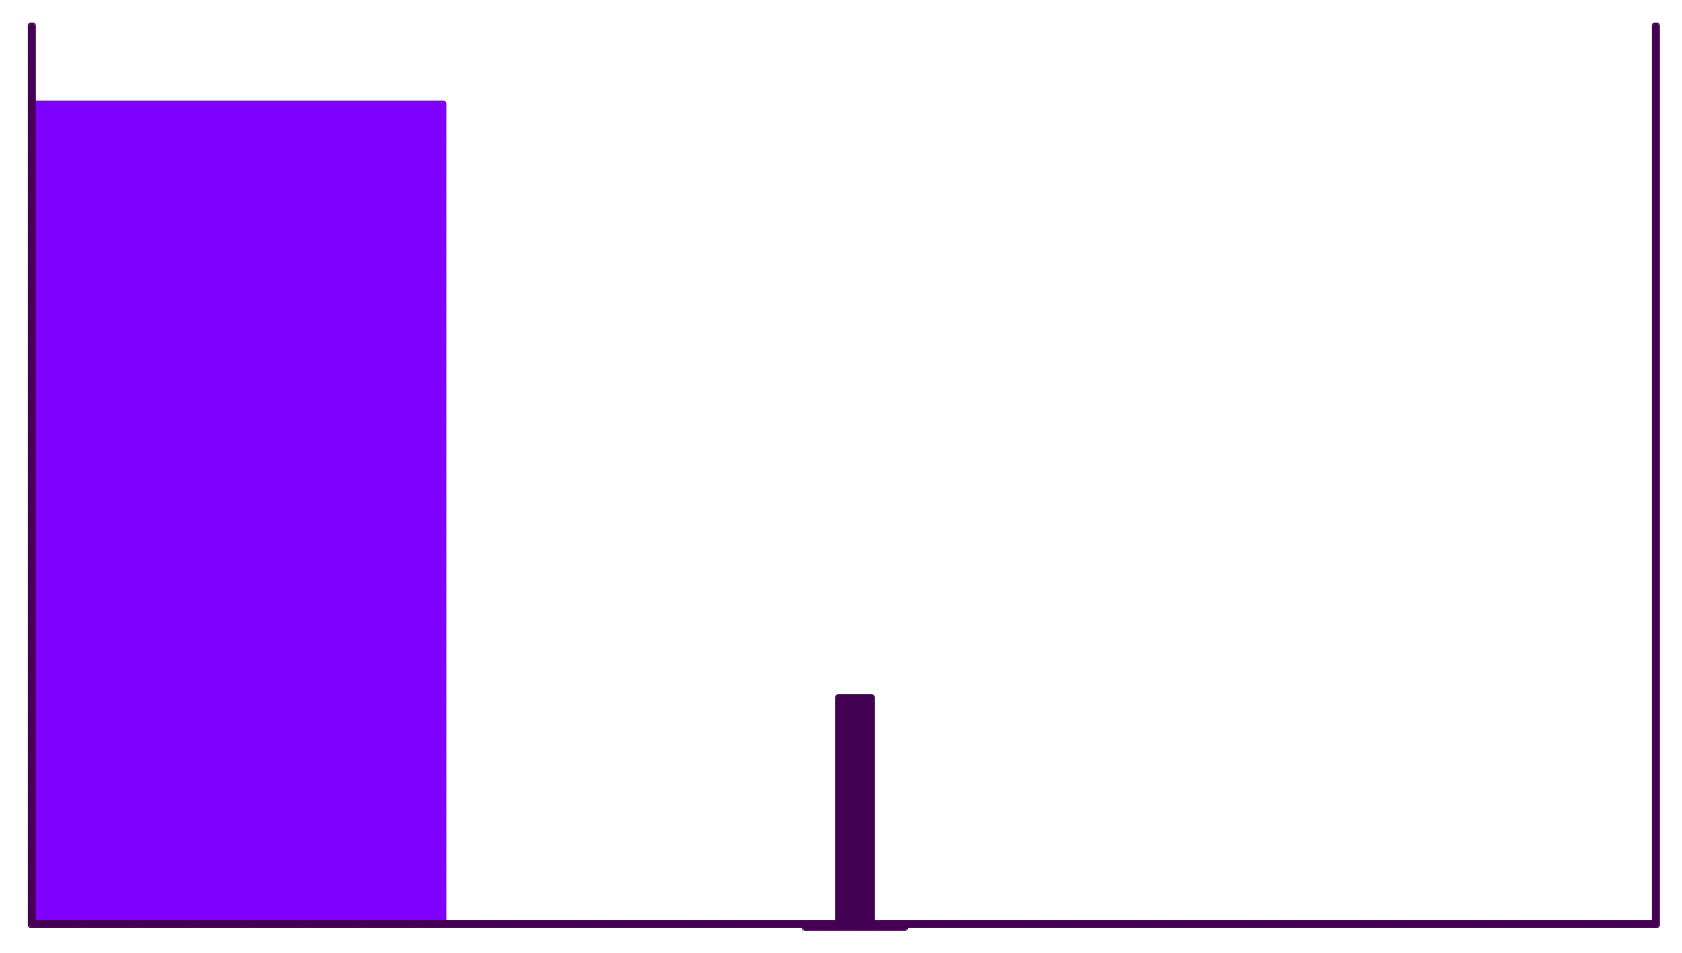
\includegraphics[scale=0.5]{figures/sun_2019_dam_breaking_flow_impacting_an_elastic_plate/snap_t_0.png}
    }
    \\
    \subfigure[]
    {
        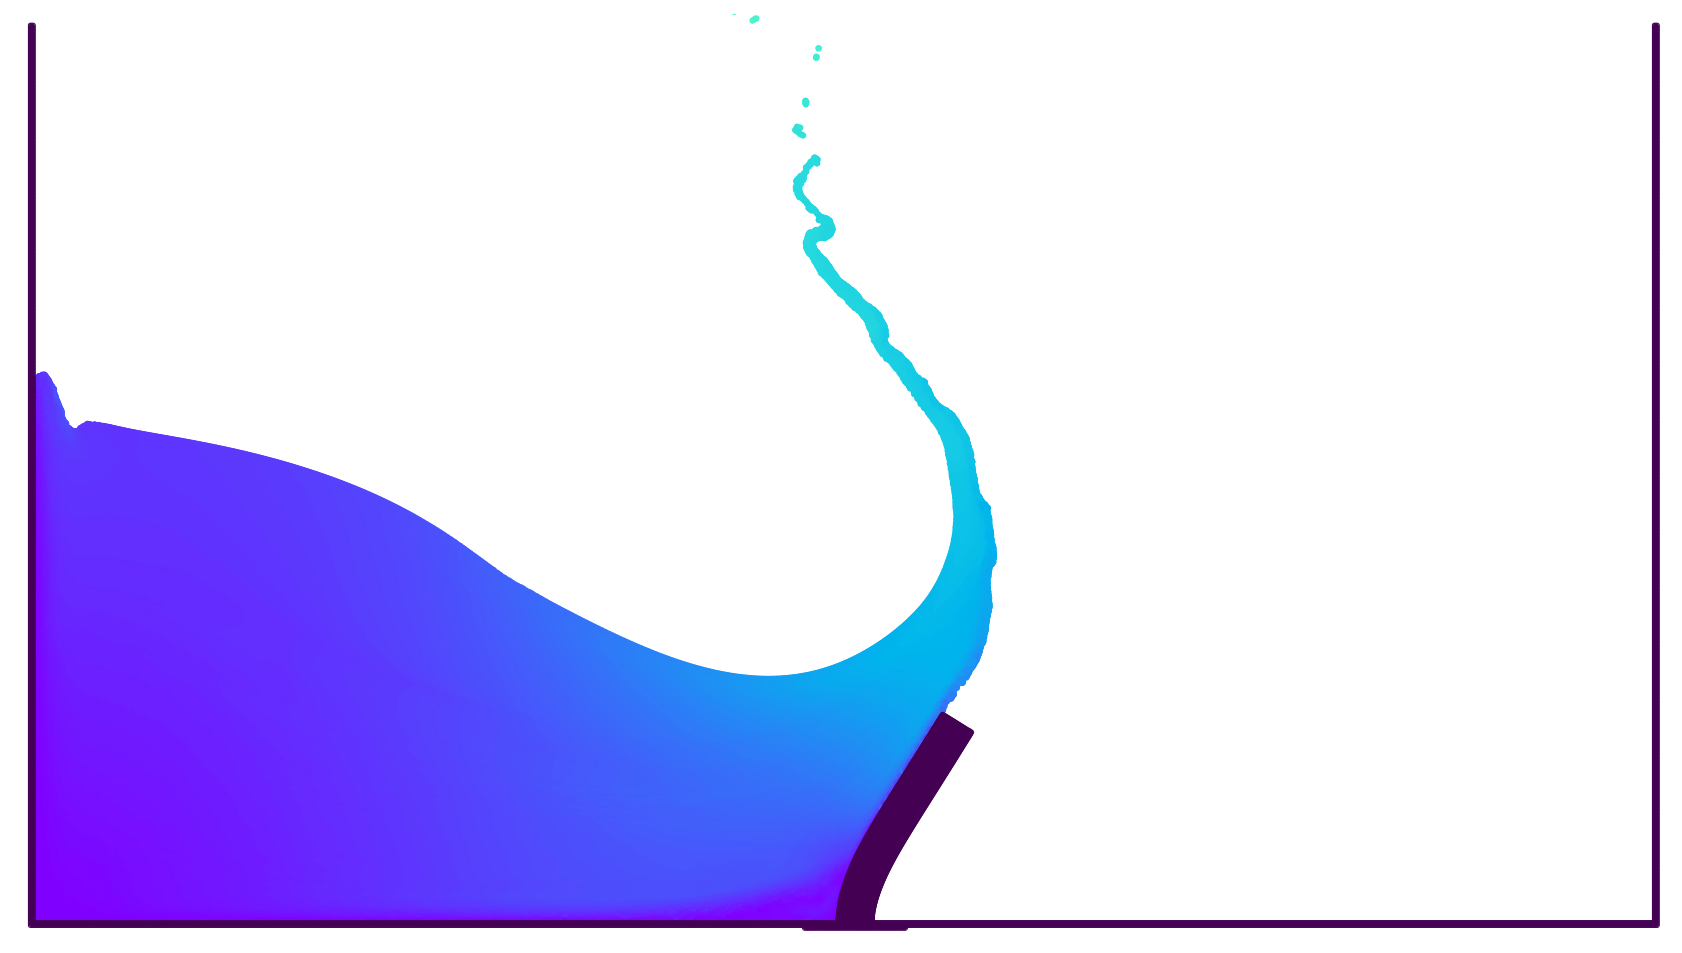
\includegraphics[scale=0.5]{figures/sun_2019_dam_breaking_flow_impacting_an_elastic_plate/snap_t_1.png}
    }
    \\
    \subfigure[]
    {
        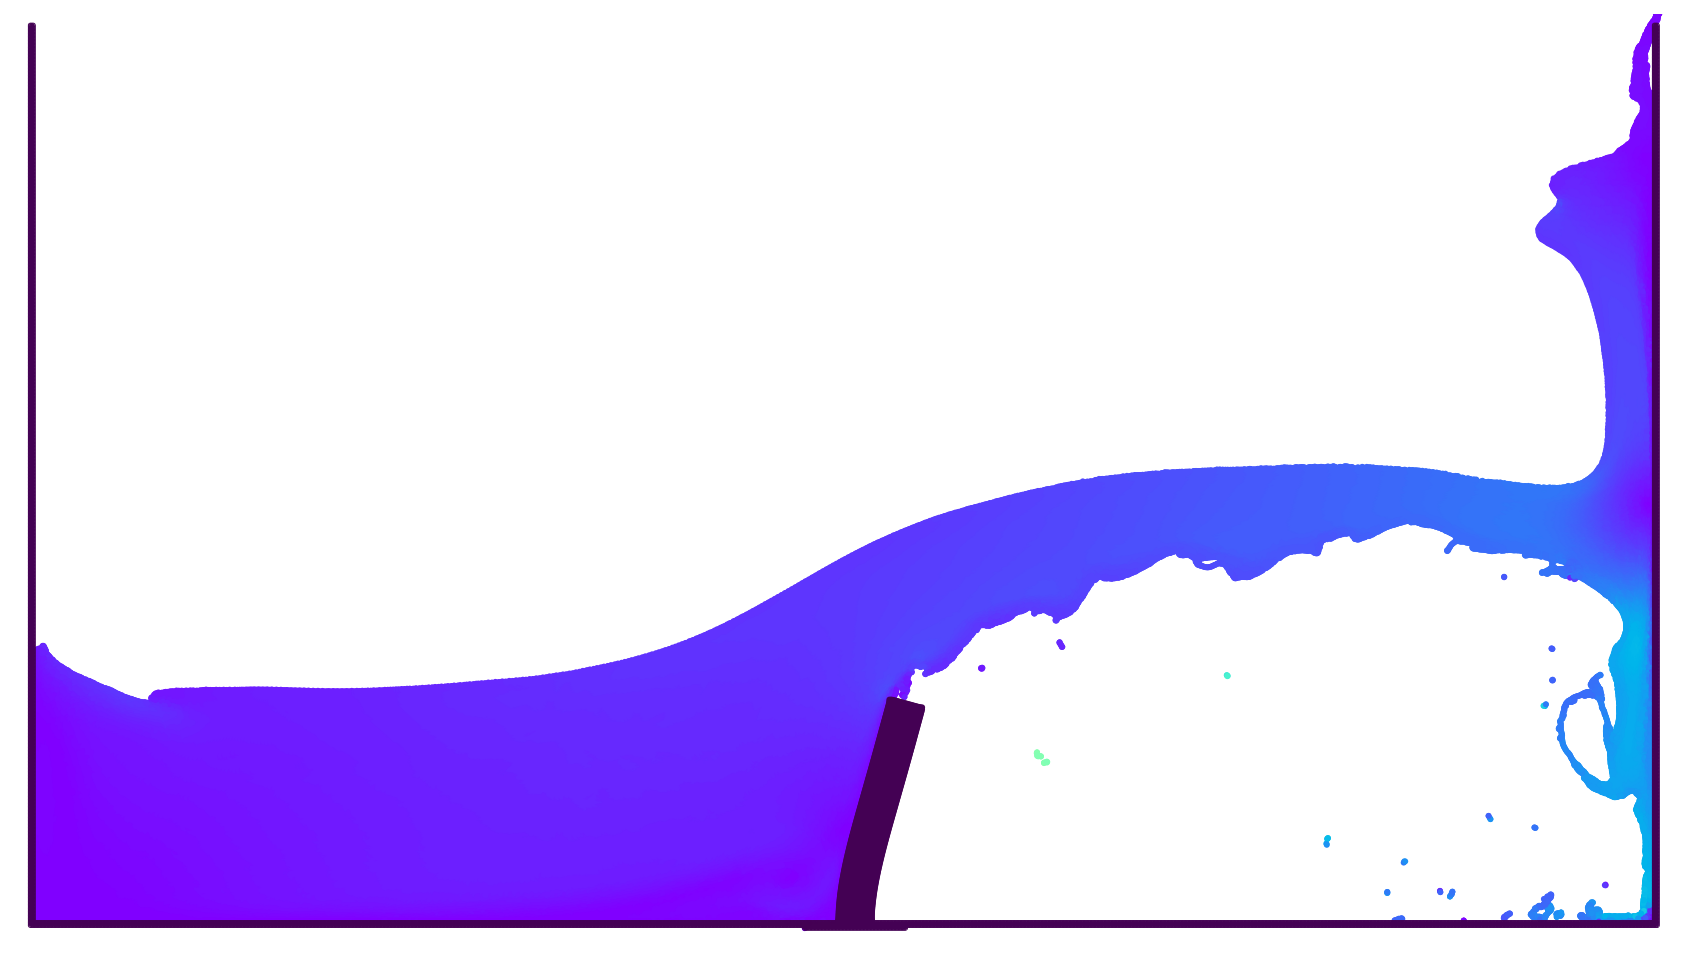
\includegraphics[scale=0.5]{figures/sun_2019_dam_breaking_flow_impacting_an_elastic_plate/snap_t_2.png}
    }
    \\
    \subfigure[]
    {
        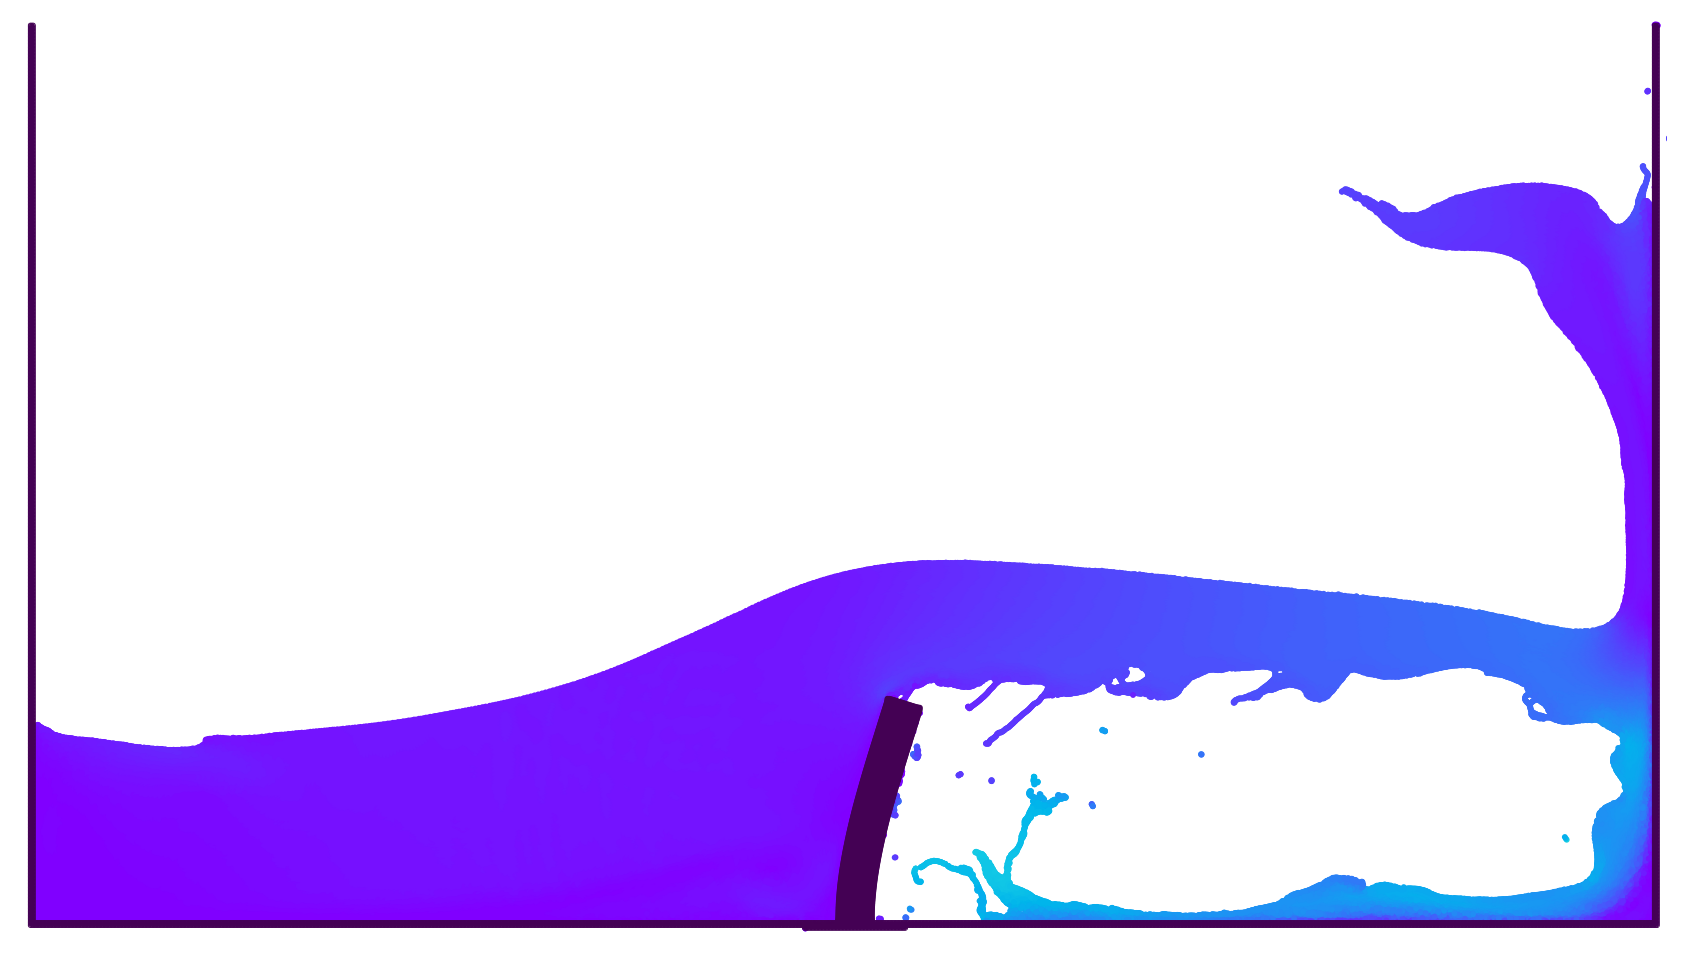
\includegraphics[scale=0.5]{figures/sun_2019_dam_breaking_flow_impacting_an_elastic_plate/snap_t_3.png}
    }
    \\
    \subfigure[]
    {
        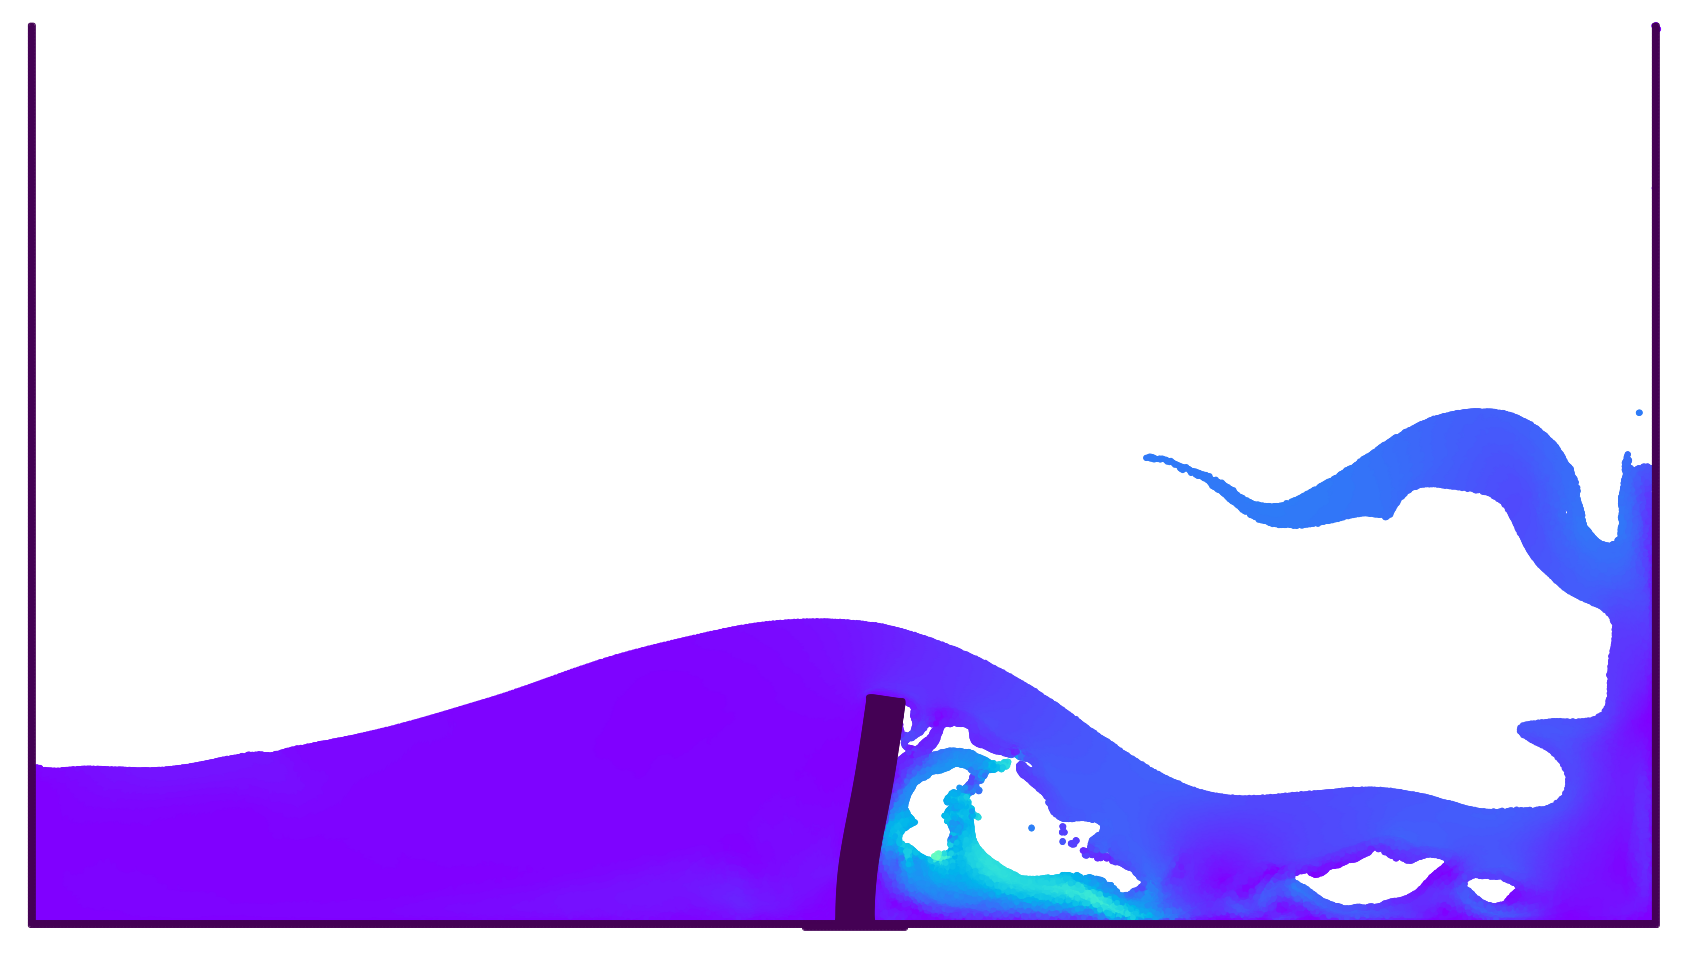
\includegraphics[scale=0.5]{figures/sun_2019_dam_breaking_flow_impacting_an_elastic_plate/snap_t_4.png}
    }
    \caption
    {
        (a) Snapshot of the fluid and the structure at different time stamps.
    }
    \label{fig:dam-breaking-onto-plate-snapshot}
\end{figure}
% \Cref{fig:dam-breaking-onto-plate-snapshot} shows snapshots of the fluid along
% with the elastic plate at different time instances. The fluid initially flows
% down the dam and hits the plate with a velocity. The plate obstructs the flow
% and the fluid will rise and hits the other end of the dam and traverses back and
% hits the plate again deforming it. This coupling between the fluid and structure
% is captured with the current scheme. From
% \cref{fig:dam-breaking-onto-plate-snapshot} we have produced a smooth particle
% distribution as well as smooth velocity profile.
\begin{figure}[H]
  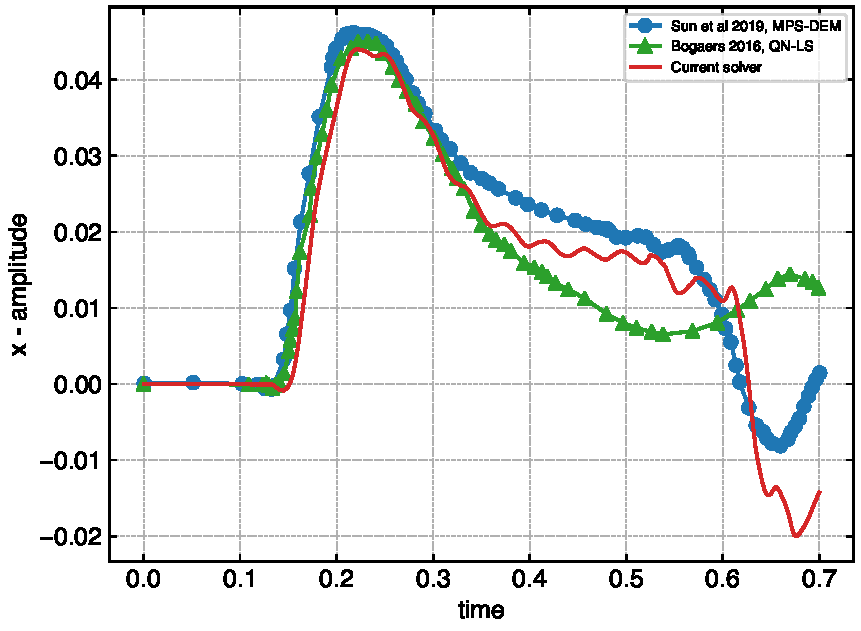
\includegraphics[scale=0.5]{figures/sun_2019_dam_breaking_flow_impacting_an_elastic_plate/x_amplitude}
  \caption{The mid-span deflection of the structure with time}
\label{fig:water-impact-plate-deflection-quantitative}
\end{figure}
% \Cref{fig:water-impact-plate-deflection-quantitative} depicts the variation of
% the displacement of the x-amplitude of the elastic beam with time. The simulated
% results are compared against variant different solvers, such as PFEM by
% Idelsohn, MPS-DEM by Sun, and a SPH variant solver by Liu. From the
% \cref{fig:water-impact-plate-deflection-quantitative}, we can see that the
% current solver is able to achieve the result up to a good approximation as other
% numerical techniques.


% ========================================================
% ========================================================
\section{\textbf{CONCLUSIONS}}\label{sec4}
% ========================================================
% ========================================================

In the current work we have coupled a unified particle method called CTVF to
handle fluid structure interaction problems. By using CTVF scheme to model both
fluid and solid phase we have eliminated many problems which are there in the
literature such as in homogeneous particle distribution in fluid phase as well
as tensile instability in solids phase. While a usual updated Lagrangian SPH
uses Gray corrections to eliminate the tensile instability and particle shifting
in fluid phase is done with tvf, we have used one set of equations to solve both
the phases and with out using any additional corrections we were able to
simulate fsi. Additionally, both phase of particles are handled in the same
frame unlike other coupling schemes in SPH, where the fluid phase follows a
updated Lagrangian model and structure phase follows a total Lagrangian. We
validated the current schemes by solving a udl problem to test the structure
equations of CTVF. And an aluminium plate over a hydrostatic tank where an
analytical solution is available is utilized to validate the fsi part of the
current solver. Finally it is applied to wave front arising due to a dam break
hitting a steady elastic plate, here the deformation of the elastic plate is
compared against the experimental results. A convergence analysis is undertaken
for both fundamental benchmarks, udl and hydrostatic tank.

For the future work, we can explore the current solves being extended to handle
the anisotropic structures. And 3D FSI problems can also be handled.


\vspace{0.5cm}
\noindent
\textbf{ACKNOWLEDGEMENTS}\\
\noindent If the authors want to acknowledge any person, institute, or facilities, it may be done here. \\

\vspace{0.5cm}
 \noindent
\textbf{NOMENCLATURE}\\

% \begin{tabular}{ccc}
% $A$ & Frontal area of rotor & [m$^2$]\\
% $Re$ & Reynolds number & -- \\
% $\epsilon$ & Dissipation & --
% \end{tabular}


\cite{wu2016coupled,
He2017coupled,
khayyer2018enhanced,
Sun2019study,
zhan2019stabilized,
wang2020scale,
ng2020coupled,
sun2021accurate,
khayyer2021multi,
long2021coupling,
peng2021coupling,
zhang2021deltasph,
sun2019fully,
hwang2014development,
zhang2021partitioned,
connor2021fluid,
nasar2019flexible,
khayyer2021coupled,
monaghan-gingold-stars-mnras-77,
sph:xsph:monaghan-jcp89,
sph:fsf:monaghan-jcp94,
zhang_hu_adams17,
PR:pysph:scipy16,
pysph,
pr:automan:2018,
monaghan-review:2005}

\bibliographystyle{amsplain}
\bibliography{FMFP2022}

\end{document}
